\documentclass[10pt]{beamer}

\usetheme[progressbar=frametitle]{metropolis}
\usepackage{appendixnumberbeamer}
\usepackage{amsmath}

\usepackage{booktabs}
\usepackage[scale=2]{ccicons}

\usepackage{pgfplots}
\usepgfplotslibrary{dateplot}

\usepackage{xspace}
\newcommand{\themename}{\textbf{\textsc{metropolis}}\xspace}

\title{67301 - MULTI ROBOT SYSTEMS - Spring 2021}
\subtitle{Final project presentation}
\date{}
\author{Tamer Ghattas}
\institute{
The Hebrew University of Jerusalem School of Computer Science and Engineering
}
% \titlegraphic{\hfill\includegraphics[height=1.5cm]{logo.pdf}}

\begin{document}

\maketitle


\section{Single-agent dirt collection}

\begin{frame}{Single-agent dirt collection}
\begin{itemize}
    \item {\bf Problem description:} collect as many as possible dirt pieces from an unknown environment without having the option of sensing the dirt. 
    \item That can be translated to: we need to cover diverse areas in the room in the shortest period of time.
    \item The problem is hard because with the time limitation we often inherit an upper bound for the area coverage.
    \item An exhaustive approach to the solution would be moving sequentially along every accessible point known from the map in hand competing a perfect coverage.
\end{itemize}
\end{frame}


\begin{frame}{Single-agent dirt collection}

We model the problem as a graph $G=(V, E)$ where the nodes $V$ represent a pixel in the map and $E$ and edge existing between every adjacent pair of pixels (nodes).


\bigskip


Our suggested solution takes the graph as input and derive goals for the robot aiming for diverse area coverage.
\end{frame}


\begin{frame}{Single-agent dirt collection}

We implemented our approach using image processing manipulations on the binary image of the given map:
\graphicspath{{images/}}
\begin{itemize}
    \item First we generate binary image from the map structure.
    \item Then we perform Euclidean Distance Transform on the image.
    \item Now, we have range of gray levels that are distributed among pixels as a function their distance of the nearest black pixel, i.e the nearest wall.
    \bigskip
    
    \begin{figure}[htp]
    \centering
    \includegraphics[height=3cm,width=4cm]{map}
    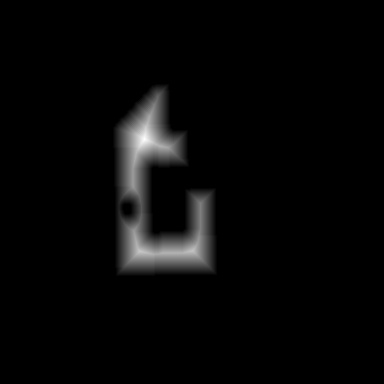
\includegraphics[height=3cm,width=4cm]{edt_img}

    \label{fig:galaxy}
\end{figure}
    
\end{itemize}
\end{frame}


\begin{frame}{Single-agent dirt collection}

\graphicspath{{images/}}
\begin{itemize}
    \item By quantizing the EDT image according to grey levels into a selected number of partitions, we get a complete partition of the room.
    \item Then, we sample from each part a number of points which become then a goals points. The robot movement is done using move-base node.
    \item Note that by increasing the resolution of the sampling we can guarantee more area coverage.
    \item In the following images, we can see the different parts and the sampled goals it yields (in orange): 
    
    \bigskip
    \begin{figure}[htp]
    % \centering
    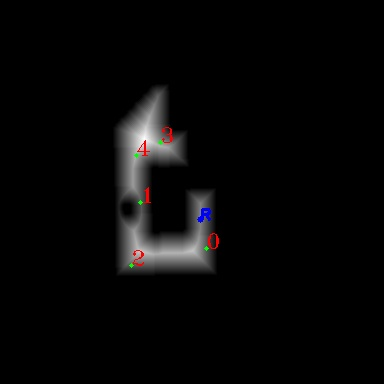
\includegraphics[height=3cm,width=3cm]{edt_img_circs_1}
    \includegraphics[height=3cm,width=3cm]{edt_img_circs_2}
    \includegraphics[height=3cm,width=3cm]{edt_img_circs_3}
    \includegraphics[height=3cm,width=3cm]{edt_img_circs_4}

    \label{fig:galaxy}
\end{figure}
    
\end{itemize}

\end{frame}


\begin{frame}{Single-agent dirt collection}
\bigskip 
We evaluated our approach by  TODO!!!
\end{frame}


\begin{frame}{Single-agent dirt collection}

\begin{itemize}
    \item This approach was the second, first I thought about using Zig-Zag pattern with a randomly sampled angle on each turn but that is prone to missing parts of certain room structures.
    \item The presented approach on average, covers all parts of the room after enough time.
    \item A good approach might be to partition the map into compact clusters and run Zig-Zag like pattern on each.
\end{itemize}

\end{frame}


\section{Single-agent inspection}
\begin{frame}{Single-agent inspection}
\begin{itemize}
    \item {\bf Problem description:} explore a room and count the number of statically positioned spheres subject to a time limit. 
    \item That can be translated to: cover all the accessible areas using the agent sensors range and register the spheres positions within the given time frame.
    \item The problem is hard because, first, exploring is a hard problem and second, detecting sphere using a low quality 2d bird view of the sensors reading is challenging.
    \item An exhaustive approach to the solution would be using BFS/DFS algorithm to map the room including the existing static objects like the spheres.
\end{itemize}
\end{frame}

\begin{frame}{Single-agent inspection}
    We model the problem as a walk-by-wall using PD controller to keep a distance from the wall and gradually increase this reserved distance after each full circle and registering the spheres positioned along the way.
    
    PD formulation:

\begin{align*} 
&\omega(t)=K_{P} e(t)+K_{P} \frac{d e}{d t}\ \ s.t\\
&\omega(t)\text{ - PD output }\\
&K_{P}\text{ - proportional gain }\\
&de\text{ - change in error value }\\
&dt\text{ - change in time } 
\end{align*}    

\end{frame}


\begin{frame}{Single-agent inspection}
We implemented our approach using PD output for movement and the local cost map  for spheres count. For every relevant sensor reading:
\graphicspath{{images/}}
\begin{itemize}
    \item Adjust linear velocity according to distance from front wall.
    \item Adjust angular velocity according PD output.
    \item Process local cost map image and detect circles using Hough transform.
    \item For each detected circle center, register centers in a set to prevent counting twice.
    \bigskip
    
    \begin{figure}[htp]
    % \centering
    \includegraphics[height=3cm,width=3cm]{gazibo.JPG}
    \includegraphics[height=3cm,width=3cm]{sphere_img_0 (4).jpg}
    \includegraphics[height=3cm,width=3cm]{sphere_img_1 (2).jpg}

    \label{fig:galaxy}
\end{figure}
    
\end{itemize}

\end{frame}


\section{Multi-agent dirt collection}

\section{Multi-agent dirt inspection}

\section{Conclusion}



\end{document}
